\chapter{IPv6-Multicast}
\label{chap:ipv6_multicast}

\section{Ejercicio 3.1}
\subsection{En los primeros 2 segundos de simulación se envían varios paquetes NS. Muestra una captura del tráfico de
paquetes en Wireshark en la que se vean las direcciones IP y MAC origen y destino de los NS enviados desde
cada uno de los nodos host[*]. (Nota: para mostrar las direcciones MAC añade dos nuevas columnas: Hw src
addr (unresolved) y Hw dest addr (unresolved). Colócalas a la derecha de las direcciones IP.) ¿De qué tipo son
las direcciones IP? ¿Cómo se construyen?}

\begin{figure}[H]
    \centering
    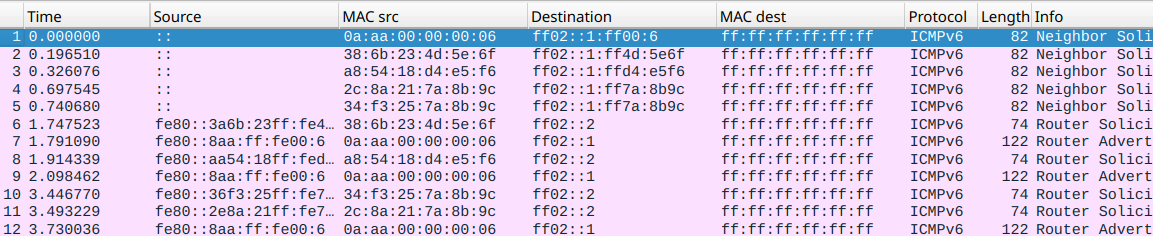
\includegraphics[width=135mm, scale=0.75]{imaxes/captura_ejer3_1.png}
    \caption{Captura MAC origen y destino host[0]}
    \label{fig:ip_mac_host0}
\end{figure}

Como las direcciones IPs de destino son multicast, en todos los hosts se ve la misma paquetería, por lo que solo subimos la captura de tráfico en el host[0].

Las direcciones, como hemos mencionado anteriormente son multicast y se construyen con el prefijo multicast link-local (FF02::1, donde FF02 quiere decir que es tipo multicast, siendo el 2 un scope de local de enlace y el ultimo 1 quiere decir todos los dispositivos, si fuera un 2 serian todos los routers). Por último tendriamos como sufijo, los 3 bytes menos significativos de la MAC del dispositivo de ese host precedido de FF.

Por ejemplo, en el primer caso tenemos como destino FF02::1:FF00:0006 donde F002::1 es como explicamos antes, el prefijo multicast link-local y como sufijo FF00:0006, donde 000006 son los 3 últimos bytes de la MAC de la interfaz del router en ese enlace (0A:AA:00:00:00:06)

\section{Ejercicio 3.2}
\subsection{¿Coincide alguna de las direcciones IP destino de los diferentes paquetes NS? ¿Por qué? ¿Qué consecuencia
tiene esto?}

Coinciden las direcciones IP del host[0] y host[2] ya que los dos tienen los 3 últimos bytes de la MAC iguales por lo que la dirección multicast se construye de la misma forma.

Con respeto a las consecuencias que puede se puede tener al haber dos direcciones multicast iguales, no es ninguna ya que los mensajes ICMPv6 de tipo NS (Neighbor Solicitation), guarda en su cabecera la dirección unicast de destino por lo que no se daría ninguún conflito (target address). Aunque no pase nada, lo normal es que las direcciones multicast de nodo solicitado (FF02::1) sean únicas.


\section{Ejercicio 3.3}
\subsection{¿Por qué se envían los NS a esas direcciones IP?}

Se envian ICMPv6 de tipo NS a esas direcciones ya que haciendolo con direcciones multicast, se puede mandar un único paquete a uno o varios destinos, de esta forma optimizamos la comunicación y reducimos el tráfico de la red para que no se congestione por lo que aumenta la eficiencia. 


\section{Ejercicio 3.4}
\subsection{¿Qué direcciones MAC destino tienen los paquetes NS anteriores? ¿Cuáles deberían tener según lo visto en
clases de teoría? (Utiliza el paquete NS que sale desde host[1] como ejemplo y escribe los 6 bytes que debería
tener la dirección MAC en formato hexadecimal.)}

\begin{figure}[H]
    \centering
    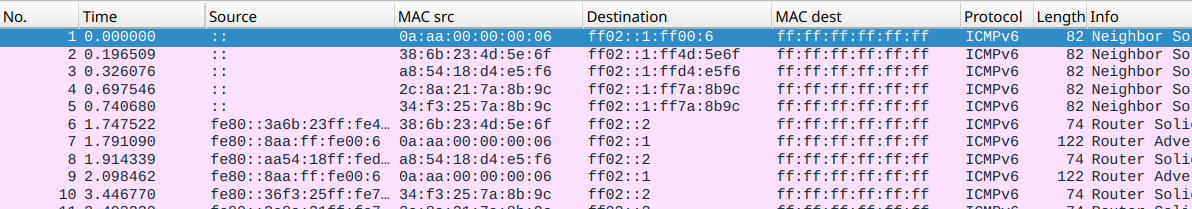
\includegraphics[width=135mm, scale=0.75]{imaxes/captura_ejer3_4.png}
    \caption{Captura MAC origen y destino paquetes NS en host[1]}
    \label{fig:ip_mac_host1}
\end{figure}

Como se puede observar en la imagen \ref{fig:ip_mac_host1}, todos los paquetes tienen como MAC destino FF:FF:FF:FF:FF:FF. Según se ha visto en la clase de teoría, las MAC tiene la estrutura 33:33:FF como prefijo de la MAC y después los 3 últimos bytes son los 3 bytes menos significativos de la dirección multicast. En este caso el destino es como dirección MAC broadcast ya que Omnet no sabe como construir este tipo de direcciones MAC como se explica en la teoría, por eso todos los hosts reciben la misma paquetería. De la otra forma cada uno recibiría su propia paquetería

\section{Ejercicio 3.5}
\subsection{¿Qué consecuencia tiene esta diferencia con respecto a lo visto en clase de teoría?}

Resulta que las consecuencias de usar dirección MAC broadcast es que todo el mundo recibe paquetes que en realidad no tendrian que recibir por lo que se sobrecarga la red. Usando la direccion MAC que se especifica en la teoria, solamente se mandaría el paquete a ese host.

\section{Ejercicio 3.6} 
\subsection{Muestra las direcciones IP y MAC destino de los mensajes RS y RA que aparecen en torno al segundo 2 de
simulación. ¿De qué tipo son las direcciones IP?}

\begin{figure}[H]
    \centering
    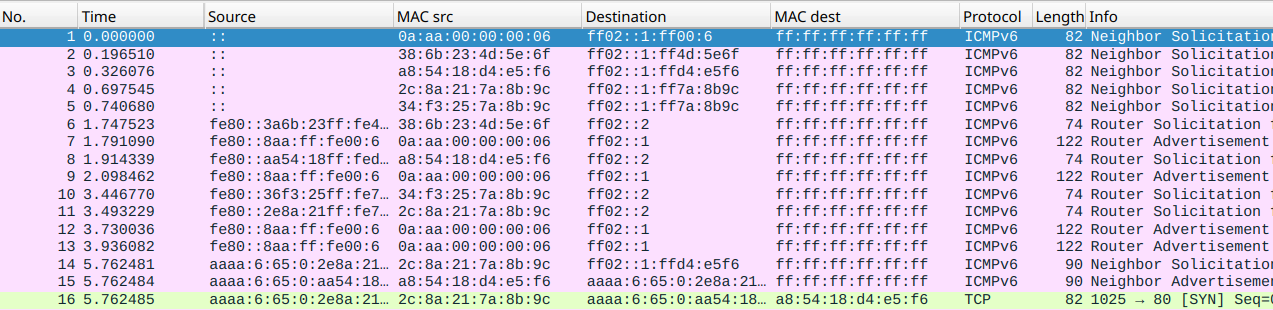
\includegraphics[width=135mm, scale=0.75]{imaxes/captura_ejer3_6.png}
    \caption{Captura paquetes RS y RA host[0]}
    \label{fig:rs_ra_h1}
\end{figure}

Como se puede observar en la imagne \ref{fig:rs_ra_h1}, en el caso de los paquetes ICPMv6 con mensaje RS tienen como dirección destino la direccion multicast FF02::2 y como MAC de destino tiene la dirección FF:FF:FF:FF:FF:FF. En este caso la dirección multicast son de este tipo ya que son direcciones a las que van dirigidos los paquetes a todos los routers de la misma red de en enlace para asi optimizar el proceso de descubrimiento de routers y no malgastar ancho de banda.

En el caso de los paquetes ICMPv6 con mensaje RA tienen como dirección destino la direccion multicast FF02::1 y como MAC de destino tiene la dirección FF:FF:FF:FF:FF:FF. En este caso la dirección multicast tiene esta estructra ya que va dirigido a todo dispositivo que está en el mismo enlace de red. 

\section{Ejercicio 3.7}
\subsection{¿Por qué el RA de respuesta a un RS no usa IP destino unicast?}

Este enfoque permite enviar la información de configuración a todos los dispositivos de la red sin necesidad de identificar la dirección específica de cada uno. Si se utilizara una dirección unicast, sería necesario conocer la dirección única de cada dispositivo, lo que resultaría poco práctico en redes grandes o cuando los dispositivos conectados pueden cambiar con frecuencia. Así de esta forma, el tráfico no se sobrecarga y resultaría todo mas eficiente.

\section{Ejercicio 3.8}
\subsection{¿Qué direcciones MAC destino deberían tener los RS según lo visto en clases de teoría? ¿Y los RA?}

La MAC destino del paquete RS debería ser 33:33:00:00:00:02, asegurando que solo los routers reciban las solicitudes de descubrimiento de nodos, y los paquetes RA deberían tener como MAC destino 33:33:00:00:00:01, por lo que así mapearía a todos los dispositivos IPv6 de esa misma red.

\section{Ejercicio 3.9}
\subsection{ Aproximadamente en t = 6 s el router envía dos NS. ¿De qué tipo son las direcciones IP destino de estos
paquetes? Explica cómo se construyen (notación IPv6 no abreviada).}

\section{Ejercicio 3.10}
\subsection{¿En qué equipos llega el segundo paquete NS enviado por el router al módulo ipv6? ¿Y al submódulo
ipv6.neighborDiscovery? ¿Por qué? Nota: para ver el recorrido del paquete en el módulo ipv6, haz doble click en
el nodo deseado y luego en el módulo ipv6. Puedes mostrar varios nodos a la vez en diferentes ventanas con
botón derecho → Open Graphical View for ‘ipv6’ una vez dentro de ese nivel.)}

\section{Ejercicio 3.11}
\subsection{¿En qué equipos llegaría el mensaje al módulo ipv6 si INET implementase direcciones MAC multicast (33-
33-xx-xx-xx-xx)? ¿Por qué?}